\documentclass[xetex,notheorems,hyperref={pdfpagelabels=true},xcolor={table},aspectratio=169]{beamer}
\usetheme{minflat}
\usepackage{booktabs}
\usepackage[scale=2]{ccicons}

\usepackage[style=american]{csquotes}

\usetikzlibrary{decorations.pathreplacing, decorations.pathmorphing,calc,arrows,positioning,patterns,fadings,shadows, arrows.meta}
\tikzset{
    %Define standard arrow tip
    >=stealth'
}


\tikzfading[name=fade right, left color=transparent!0, right color=transparent!100]
\tikzfading[name=fade left, left color=transparent!100, right color=transparent!0]
\tikzfading[name=fade out, inner color=transparent!0, outer color=transparent!100]

%define hatched pattern
\pgfdeclarepatternformonly{south west lines}{\pgfqpoint{-0pt}{-0pt}}{\pgfqpoint{3pt}{3pt}}{\pgfqpoint{3pt}{3pt}}{
        \pgfsetlinewidth{0.4pt}
        \pgfpathmoveto{\pgfqpoint{0pt}{0pt}}
        \pgfpathlineto{\pgfqpoint{3pt}{3pt}}
        \pgfpathmoveto{\pgfqpoint{2.8pt}{-.2pt}}
        \pgfpathlineto{\pgfqpoint{3.2pt}{.2pt}}
        \pgfpathmoveto{\pgfqpoint{-.2pt}{2.8pt}}
        \pgfpathlineto{\pgfqpoint{.2pt}{3.2pt}}
        \pgfusepath{stroke}}

\setbeamercovered{invisible}

%%% enable notes on second screen
%\usepackage{pgfpages}
%\setbeameroption{show notes on second screen=right}
%\setbeamertemplate{note page}[compress]

\definecolor{proofgreen}{RGB}{233,4,105}
\definecolor{implementation}{RGB}{41,2,81}
	
%%%%%%%%%%%%%%%%%%%%%%%%%%%%%%%%%%%%%%%%%%%%%%%%%%%
%%%%	define content of title page
%%%%%%%%%%%%%%%%%%%%%%%%%%%%%%%%%%%%%%%%%%%%%%%%%%%
\def\talkTitle{Conception, implémentation et preuve d’un service de transfert de flot d’exécution au sein d’un noyau de système d’exploitation}
\def\talkSubtitle{Soutenance de thèse}
\def\talkKeywords{Keywords}

%% Define meta data of pdf
\hypersetup{
    pdftitle={Slides to talk - \talkTitle},
	pdfsubject={\talkTitle},
	pdfauthor={Florian Vanhems},
	pdfkeywords={\talkKeywords},
	colorlinks=false
}


%%%%%%%%%%%%%%%%%%%%%%%%%%%%%%%%%%%%%%%%%%%%%%%%%%%
%%%%	set content of title page
%%%%%%%%%%%%%%%%%%%%%%%%%%%%%%%%%%%%%%%%%%%%%%%%%%%
\title{\talkTitle}  
\subtitle{\textbf{\talkSubtitle}}
\author{Florian Vanhems -- florian.vanhems@univ-lille.fr}
\date{Jeudi 2 Mars 2023}
\institute{%
	\centering
	\def\svgwidth{.35\textwidth}
	\input{./images/logo_ulille.pdf_tex}\\
}

%%%%%%%%%%%%%%%%%%%%%%%%%%%%%%%%%%%%%%%%%%%%%%%%%%%
%%%%	theorem tools, theorem and proof styles
%%%%%%%%%%%%%%%%%%%%%%%%%%%%%%%%%%%%%%%%%%%%%%%%%%%
\setbeamertemplate{theorem}[ams style]
%\setbeamertemplate{theorems}[numbered]

\newcounter{chapter}
\setcounter{chapter}{1}
\theoremstyle{plain}
\newtheorem{theorem}{Théorème}[section]
\newtheorem{lemma}[theorem]{Lemme}
\newtheorem{proposition}[theorem]{Proposition}
\newtheorem{corollary}[theorem]{Corollaire}

\theoremstyle{definition}
\newtheorem{conclusion}[theorem]{Conclusion}
\newtheorem*{definition}{Définition}
\newtheorem*{remark}{Remarque}
\newtheorem*{dummyblock}{dummyblock}

\theoremstyle{example}
\newtheorem{example}[theorem]{Exemple}

\newenvironment<>{dummyblock}[1]{%
	\setbeamercolor{block title}{fg=white,bg=white}%
	\setbeamercolor{block body}{fg=normal text.fg,bg=white}%
	\begin{block}#2{#1}}{\end{block}}

\begin{document}
\renewcommand{\leq}{\leqslant}
\renewcommand{\geq}{\geqslant}

\renewcommand\theta\vartheta


%%%%%%%%%%%%%%%%%%%%%%%%%%%%%%%%%%%%%%%%%%%%%%%%%%%
%%%%	title page
%%%%%%%%%%%%%%%%%%%%%%%%%%%%%%%%%%%%%%%%%%%%%%%%%%%
\begin{frame}[plain]
	\titlepage
\end{frame}

%%%%%%%%%%%%%%%%%%%%%%%%%%%%%%%%%%%%%%%%%%%%%%%%%%%
%%%%	Introduction
%%%%%%%%%%%%%%%%%%%%%%%%%%%%%%%%%%%%%%%%%%%%%%%%%%%
\section{Introduction}

\begin{frame}[fragile]
	\frametitle{Contexte général et portée des travaux}
	Sécurité informatique de systèmes critiques\\
	Dysfonctionnement provoque la mise en péril de vies humaines ou engendre des coûts effarants
	\begin{itemize}
		\item Transport
		\item Énergie
		\item Spatial
	\end{itemize}

	Preuve de propriétés formelles sur le logiciel embarqué dans ces systèmes 
\end{frame}

\begin{frame}[fragile]
	\frametitle{Pip, un noyau minimal aux garanties fortes}
	\begin{itemize}
		\item{Permet de créer des partitions de mémoire isolées les unes des autres}
		\item{Isolation rendue possible par un dispositif matériel (MMU ou MPU selon les systèmes)}
		\item{Muni d'une preuve formelle de préservation de l'isolation (bonne configuration du matériel)}
		\item{Support des architectures x86 et Armv7}
	\end{itemize}
\end{frame}

\begin{frame}[fragile]
	\frametitle{L'arbre de partition de Pip}
	\begin{center}
		\begin{tikzpicture}[>=triangle 45,font=\sffamily, every text node part/.style={align=center}, scale=0.55, every node/.style={transform shape}]

\onslide<1> {
	\node[draw, thick, minimum width=4cm, minimum height=2cm] (pip) at (0, -3) {Pip};

	\draw[dashed] (-10.5, -1.5) -- (7, -1.5);
	\node at (-9, -1) {Espace utilisateur};	
	\node at (-9, -2) {Espace privilégié};	

	\node[draw, thick, minimum width=4cm, minimum height=2cm] (root) at (0, 0) {Multiplexer};
	\node[draw, thick, minimum width=4cm, minimum height=2cm] (child1) at (-5, 3) {Linux};
	\node[draw, thick, minimum width=4cm, minimum height=2cm] (child2) at (5, 3) {FreeRTOS};

	\node[draw, thick, minimum width=4cm, minimum height=2cm] (gchild) at (-5, 6) {Shell};

	\draw[semithick] (root) -- (child1);
	\draw[semithick] (root) -- (child2);
	\draw[semithick] (child1) -- (gchild);

}

\onslide<2> {
	\node[draw, thick, minimum width=4cm, minimum height=2cm] (pip) at (0, -3) {Pip};

	\draw[dashed] (-10.5, -1.5) -- (7, -1.5);
	\node at (-9, -1) {Espace utilisateur};	
	\node at (-9, -2) {Espace privilégié};	

	\node[draw, thick, minimum width=4cm, minimum height=2cm] (root) at (0, 0) {Multiplexer};
	\node[opacity=0.3, draw, thick, minimum width=4cm, minimum height=2cm] (child1) at (-5, 3) {Linux};
	\node[opacity=0.3, draw, thick, minimum width=4cm, minimum height=2cm] (child2) at (5, 3) {FreeRTOS};

	\node[opacity=0.3, draw, thick, minimum width=4cm, minimum height=2cm] (gchild) at (-5, 6) {Shell};

	\draw[opacity=0.3, semithick] (root) -- (child1);
	\draw[opacity=0.3, semithick] (root) -- (child2);
	\draw[opacity=0.3, semithick] (child1) -- (gchild);

%%%%%%%%%%%%%%%%%%%%%%%%%%%%%%%%%%%%%%%%%%%%%%%%%%%%%%%%%%%%%%%%%%
	\node[left=2cm of root] (root_text) {La partition \emph{racine}\\a accès à l'intégralité de la mémoire du système};
	\draw[->, semithick] (root_text) -- (root);
}

\onslide<3> {
	\node[draw, thick, minimum width=4cm, minimum height=2cm] (pip) at (0, -3) {Pip};

	\draw[dashed] (-10.5, -1.5) -- (7, -1.5);
	\node at (-9, -1) {Espace utilisateur};	
	\node at (-9, -2) {Espace privilégié};	

	\node[draw, thick, minimum width=4cm, minimum height=2cm] (root) at (0, 0) {Multiplexer};
	\node[draw, thick, minimum width=4cm, minimum height=2cm] (child1) at (-5, 3) {Linux};
	\node[opacity=0.3, draw, thick, minimum width=4cm, minimum height=2cm] (child2) at (5, 3) {FreeRTOS};
	\node[opacity=0.3, draw, thick, minimum width=4cm, minimum height=2cm] (gchild) at (-5, 6) {Shell};

	\draw[semithick] (root) -- (child1);
	\draw[opacity=0.3, semithick] (root) -- (child2);
	\draw[opacity=0.3, semithick] (child1) -- (gchild);

	\node[below=0cm of root] (root_text) {Partition \emph{racine}};
%%%%%%%%%%%%%%%%%%%%%%%%%%%%%%%%%%%%%%%%%%%%%%%%%%%%%%%%%%%%%%%%%%
	\node[left=0.75cm of root] (child1_text) {Une partition \emph{enfant}\\créée à partir de la mémoire\\de la partition racine};
	\draw[->, semithick] (child1_text) -- (child1.240);

}

\onslide<4> {
	\node[draw, thick, minimum width=4cm, minimum height=2cm] (pip) at (0, -3) {Pip};

	\draw[dashed] (-10.5, -1.5) -- (7, -1.5);
	\node at (-9, -1) {Espace utilisateur};	
	\node at (-9, -2) {Espace privilégié};	

	\node[draw, thick, minimum width=4cm, minimum height=2cm] (root) at (0, 0) {Multiplexer};
	\node[opacity=0.3, draw, thick, minimum width=4cm, minimum height=2cm] (child1) at (-5, 3) {Linux};
	\node[draw, thick, minimum width=4cm, minimum height=2cm] (child2) at (5, 3) {FreeRTOS};

	\node[opacity=0.3, draw, thick, minimum width=4cm, minimum height=2cm] (gchild) at (-5, 6) {Shell};

	\draw[opacity=0.3, semithick] (root) -- (child1);
	\draw[semithick] (root) -- (child2);
	\draw[opacity=0.3, semithick] (child1) -- (gchild);

	\node[below=0cm of root] (root_text) {Partition \emph{racine}};
%%%%%%%%%%%%%%%%%%%%%%%%%%%%%%%%%%%%%%%%%%%%%%%%%%%%%%%%%%%%%%%%%%
	\node[above=1.5cm of child2] (child1_text) {Une autre partition \emph{enfant}\\créée à partir de la mémoire\\de la partition racine};
	\draw[->, semithick] (child1_text) -- (child2);

}

\onslide<5> {
	\node[draw, thick, minimum width=4cm, minimum height=2cm] (pip) at (0, -3) {Pip};

	\draw[dashed] (-10.5, -1.5) -- (7, -1.5);
	\node at (-9, -1) {Espace utilisateur};	
	\node at (-9, -2) {Espace privilégié};	

	\node[draw, thick, minimum width=4cm, minimum height=2cm] (root) at (0, 0) {Multiplexer};
	\node[draw, thick, dotted, minimum width=4cm, minimum height=2cm] (child1) at (-5, 3) {Linux};
	\node[draw, thick, dotted, minimum width=4cm, minimum height=2cm] (child2) at (5, 3) {FreeRTOS};

	\node[opacity=0.3, draw, thick, minimum width=4cm, minimum height=2cm] (gchild) at (-5, 6) {Shell};

	\draw[->, semithick, color=green!60] (root) -- (child1);
	\draw[->, semithick, color=green!60] (root) -- (child2);
	\draw[opacity=0.3, semithick] (child1) -- (gchild);

	\node[below=0cm of root] (root_text) {Partition \emph{racine}};
%%%%%%%%%%%%%%%%%%%%%%%%%%%%%%%%%%%%%%%%%%%%%%%%%%%%%%%%%%%%%%%%%%
	\node[left=1cm of root] (root_text2) {Le \emph{parent} des partitions enfants\\a toujours accès à la mémoire\\partagée avec ses enfants};

}

\onslide<6> {
	\node[draw, thick, minimum width=4cm, minimum height=2cm] (pip) at (0, -3) {Pip};

	\draw[dashed] (-10.5, -1.5) -- (7, -1.5);
	\node at (-9, -1) {Espace utilisateur};	
	\node at (-9, -2) {Espace privilégié};	

	\node[draw, thick, dotted, minimum width=4cm, minimum height=2cm] (root) at (0, 0) {Multiplexer};
	\node[draw, thick, minimum width=4cm, minimum height=2cm] (child1) at (-5, 3) {Linux};
	\node[draw, thick, minimum width=4cm, minimum height=2cm] (child2) at (5, 3) {FreeRTOS};

	\node[opacity=0.3, draw, thick, minimum width=4cm, minimum height=2cm] (gchild) at (-5, 6) {Shell};

	\draw[<-, semithick, color=red!60] (root) -- (child1);
	\draw[<-, semithick, color=red!60] (root) -- (child2);
	\draw[opacity=0.3, semithick] (child1) -- (gchild);

	\node[below=0cm of root] (root_text) {Partition \emph{racine}};
%%%%%%%%%%%%%%%%%%%%%%%%%%%%%%%%%%%%%%%%%%%%%%%%%%%%%%%%%%%%%%%%%%
	\node[above=0.5cm of root] (child1_text) {Les partitions enfants \emph{n'ont pas accès} à la\\mémoire qui ne leur a pas été partagée};
}

\onslide<7> {
	\node[draw, thick, minimum width=4cm, minimum height=2cm] (pip) at (0, -3) {Pip};

	\draw[dashed] (-10.5, -1.5) -- (7, -1.5);
	\node at (-9, -1) {Espace utilisateur};	
	\node at (-9, -2) {Espace privilégié};	

	\node[opacity=0.3, draw, thick, minimum width=4cm, minimum height=2cm] (root) at (0, 0) {Multiplexer};
	\node[draw, thick, minimum width=4cm, minimum height=2cm] (child1) at (-5, 3) {Linux};
	\node[draw, thick, minimum width=4cm, minimum height=2cm] (child2) at (5, 3) {FreeRTOS};

	\node[opacity=0.3, draw, thick, minimum width=4cm, minimum height=2cm] (gchild) at (-5, 6) {Shell};

	\draw[opacity=0.3, semithick] (root) -- (child1);
	\draw[opacity=0.3, semithick] (root) -- (child2);
	\draw[opacity=0.3, semithick] (child1) -- (gchild);
	\draw[<->, semithick, color=red!60] (child1) -- node[color=black, midway, above=1cm] {Une partition enfant \emph{ne peut pas accéder} à la mémoire d'une\\autre partition enfant (la mémoire partagée est \emph{disjointe})} (child2);

	\node[opacity=0.3, below=0cm of root] (root_text) {Partition \emph{racine}};
%%%%%%%%%%%%%%%%%%%%%%%%%%%%%%%%%%%%%%%%%%%%%%%%%%%%%%%%%%%%%%%%%%
}

\onslide<8> {
	\node[draw, thick, minimum width=4cm, minimum height=2cm] (pip) at (0, -3) {Pip};

	\draw[dashed] (-10.5, -1.5) -- (7, -1.5);
	\node at (-9, -1) {Espace utilisateur};	
	\node at (-9, -2) {Espace privilégié};	

	\node[draw, thick, minimum width=4cm, minimum height=2cm] (root) at (0, 0) {Multiplexer};
	\node[draw, thick, minimum width=4cm, minimum height=2cm] (child1) at (-5, 3) {Linux};
	\node[draw, thick, minimum width=4cm, minimum height=2cm] (child2) at (5, 3) {FreeRTOS};

	\node[opacity=0.3, draw, thick, minimum width=4cm, minimum height=2cm] (gchild) at (-5, 6) {Shell};

	\draw[opacity=0.3, semithick] (root) -- (child1);
	\draw[opacity=0.3, semithick] (root) -- (child2);
	\draw[opacity=0.3, semithick] (child1) -- (gchild);

	\draw[<->, semithick, color=red!60] (child1) -- (child2);
	\draw[<-, semithick, color=red!60] (root.175) -- (child1.270);
	\draw[<-, semithick, color=red!60] (root.5) -- (child2.270);
	\draw[->, semithick, color=green!60] (root) -- (child1);
	\draw[->, semithick, color=green!60] (root) -- (child2);

	\node[below=0cm of root] (root_text) {Partition \emph{racine}};
%%%%%%%%%%%%%%%%%%%%%%%%%%%%%%%%%%%%%%%%%%%%%%%%%%%%%%%%%%%%%%%%%%
}
\end{tikzpicture}

	\end{center}
\end{frame}

\begin{frame}[fragile]
	\frametitle{L'architecture de Pip}
	\begin{itemize}
		\item{Code des services écrit en Gallina, grâce à un shallow embedding de C}
		\item{Le code des services est traduit en C grâce à un compilateur (Digger ou $\partial x$)}
		\item{Services ensuite compilé avec le reste du noyau écrit en C et en assembleur}
		\item{Les preuves portent directement sur le code des services, dévelopées dans l'assistant de preuve Coq}
		(Faire un schéma)
	\end{itemize}
\end{frame}

\begin{frame}[fragile]
	\frametitle{Historique des travaux sur le projet Pip}
	Première génération de doctorants :
	\begin{itemize}
		\item{Aspect système : conception du noyau}
		\item{Aspect vérification : code des services et preuve}
		\item{Aspect embarqué : travaux sur la cohabitation d'entités différentes au sein du système}
	\end{itemize}

	Manque cependant un service robuste de transfert de flot d'exécution entre les partitions
\end{frame}

\begin{frame}[fragile]
	\frametitle{Contributions de la thèse}
	\begin{itemize}
		\item{Service de transfert de flot d'exécution entre les partitions}
		\item{Développement d'un ordonnanceur Earliest Deadline First dans une partition}
		\item{Amélioration de l'architecture de Pip découplant le code des modèles d'isolation}
	\end{itemize}
\end{frame}

\begin{frame}
	\tableofcontents
\end{frame}

%%%%%%%%%%%%%%%%%%%%%%%%%%%%%%%%%%%%%%%%%%%%%%%%%%%
%%%%	Service de transfert de flot de controle
%%%%%%%%%%%%%%%%%%%%%%%%%%%%%%%%%%%%%%%%%%%%%%%%%%%

\section{Service de transfert de flot d'exécution}

\begin{frame}[fragile]
	\frametitle{Motivations}
	\begin{itemize}
		\item{Gérer les cas limites non gérés par l'ancienne implémentation}
		\item{Compléter la preuve de préservation de l'isolation des services fournis par Pip}
		\item{Éprouver la méthodologie de Pip}
	\end{itemize}
\end{frame}

\begin{frame}[fragile]
	\frametitle{Quels objectifs ?}
	\begin{itemize}
		\item{Gérer les fautes et interruptions}
		\item{Minimiser le nombre de lignes de code pour faciliter la preuve de maintient de l'isolation}
		\item{Ne pas être lié à une architecture spécifique}
	\end{itemize}
\end{frame}

\begin{frame}[fragile]
	\frametitle{Transferts de flot d'exécution explicites au sein de Pip}

	\begin{center}
		\begin{tikzpicture}[>=triangle 45,font=\sffamily, every text node part/.style={align=center}, scale=0.6, every node/.style={transform shape}]
	\onslide<1> {
		\node[opacity=0.3, draw, thick, minimum width=4cm, minimum height=2cm] (root) at (0, 0) {Multiplexer};
		\node[draw, thick, minimum width=4cm, minimum height=2cm] (child1) at (-4, 4) {Linux};
		\node[opacity=0.3, draw, thick, minimum width=4cm, minimum height=2cm] (child2) at (4, 4) {FreeRTOS};
	
		\node[draw, thick, minimum width=4cm, minimum height=2cm] (gchild) at (-4, 8) {Shell};
	
		\draw[opacity=0.3, semithick] (root) -- (child1);
		\draw[opacity=0.3, semithick] (root) -- (child2);
		\draw[semithick] (child1) -- (gchild);
	
		\draw[<-, dashed] (child1.west) to [out=135, in=225] node [midway, left] {asks to open a file} (gchild.west);
	}
	\onslide<2> {	
		\node[opacity=0.3, draw, thick, minimum width=4cm, minimum height=2cm] (root) at (0, 0) {Multiplexer};
		\node[draw, thick, minimum width=4cm, minimum height=2cm] (child1) at (-4, 4) {Linux};
		\node[opacity=0.3, draw, thick, minimum width=4cm, minimum height=2cm] (child2) at (4, 4) {FreeRTOS};
	
		\node[draw, thick, minimum width=4cm, minimum height=2cm] (gchild) at (-4, 8) {Shell};
	
		\draw[opacity=0.3, semithick] (root) -- (child1);
		\draw[opacity=0.3, semithick] (root) -- (child2);
		\draw[semithick] (child1) -- (gchild);
	
		\draw[<-, dashed, opacity=0.3] (child1.west) to [out=135, in=225] node [midway, left, opacity=0.3] {asks to open a file} (gchild.west);
		\draw[->, dashed] (child1.east) to [out=45 , in=315] node [midway, right] {file is opened} (gchild.east);
	}
\end{tikzpicture}

	\end{center}
\end{frame}

%-----------------------------------------------------------
\subsection{Un nouveau service pour les transferts explicites}

\begin{frame}[fragile]
	\frametitle{Idée principale : la \emph{VIDT}}
	\begin{center}
		\begin{tikzpicture}
\node[minimum width=3cm, minimum height=3cm] (vidt) at (0,0) {};
\node[above=0.1cm of vidt] {VIDT d'une partition};
%\draw[dashed] (3.5, -1.5) -- (3.5, 1.5);
%\draw[dashed] (6.5, -1.5) -- (6.5, 1.5);
\node[draw, semithick, minimum width=3cm, minimum height=0.5cm] (ctx_ptr1) at (0,1.30) {@ctx};
\node[left=0.2cm of ctx_ptr1, minimum height=0.5cm] (top_number) {\texttt{0}};
\node[above=0.1cm of top_number] {N°.};
\node[draw, semithick, below=-0.01cm of ctx_ptr1, minimum width=3cm, minimum height=0.5cm] (ctx_ptr2) {@ctx};
\node[left=0.2cm of ctx_ptr2] {\texttt{1}};
\node[minimum width=3cm, minimum height=0.5cm] (dots) at (0,-0.2) {$\vdots$};
\node[left=0.2cm of dots] {$\vdots$};
\node[draw, minimum width=1cm, minimum height=1cm] (ctx) at (5.5, 0.5) {};
\node[inner sep=0pt, fill opacity=1] at (ctx) {
\includegraphics[width=1cm]{images/gray_context.png}};
\node[draw, semithick, below=1.5cm of ctx_ptr2, minimum width=3cm, minimum height=0.5cm] (ctx_ptr3) {@ctx};
\node[left=0.1cm of ctx_ptr3] {\texttt{255}};
\node[below=0.02cm of ctx] {Contexte d'exécution};
%\node[above=0.6cm of ctx] {Partition memory};
\node[draw, color=black!25, pattern color=black!25, minimum width=1cm, minimum height=1cm] (ctx2) at (4, 2.3) {};
\node[inner sep=0pt, fill opacity=1] at (ctx2) {
\includegraphics[width=1cm]{images/gray_context.png}};
\node[inner sep=0pt, opacity=0.75, fill=white, minimum width=1cm, minimum height=1cm] at (ctx2) {};
\node[draw, color=black!25, pattern color=black!25, minimum width=1cm, minimum height=1cm] (ctx3) at (4.7, -1.9) {};
\node[inner sep=0pt, fill opacity=1] at (ctx3) {
\includegraphics[width=1cm]{images/gray_context.png}};
\node[inner sep=0pt, opacity=0.75, fill=white, minimum width=1cm, minimum height=1cm] at (ctx3) {};
%%%%%%%%%%%%%%%%%%%%%%%%%%%%%%%%%%%%%%%%%%%%%%%%%%%%%%%%%%%%%%%
\draw[dashed, semithick] (ctx_ptr2.south west) -- (ctx_ptr3.north west);
\draw[dashed, semithick] (ctx_ptr2.south east) -- (ctx_ptr3.north east);
\draw[->, color=black!25] (ctx_ptr1.east) -- (ctx2.west);
\draw[->] (ctx_ptr2.east) -- (ctx.west);
\draw[->, color=black!25] (ctx_ptr3.east) -- (ctx3.west);
\end{tikzpicture}

	\end{center}
\end{frame}

\begin{frame}[fragile]
	\frametitle{Illustration du fonctionnement du service}
	\begin{center}
		\begin{tikzpicture}[>=triangle 45,font=\sffamily, every text node part/.style={align=center}, every node/.style={transform shape}]

%% CPU box
	\node[minimum width=0.8cm, minimum height=0.8cm] (cpu) at (0, 0) {};
%\node[draw, ultra thin, drop shadow, fill=white, minimum height=1.3cm, minimum width=1.3cm] (cpu) at (0, 0) {};
%% CPU label
%\node[above=0.1cm of cpu] {\scriptsize{CPU}};

\onslide<1-> {
	%% CPU
	\node[inner sep=0pt, fill opacity=1] at (cpu) {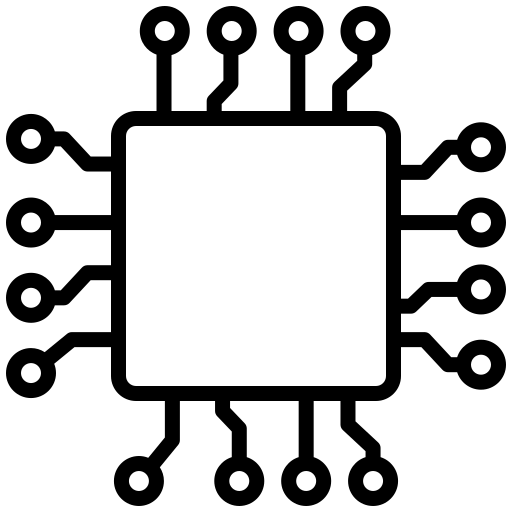
\includegraphics[width=1.5cm]{images/cpu.png}};
	%% Kernel box
	\node[draw, ultra thin, drop shadow, fill=white, minimum height=2cm, minimum width=0.8cm, above=0.7cm of cpu] (kern_stack) {};
	%% Kernel box label
	\node[above=0.1cm of kern_stack] {\scriptsize{Pile noyau}};
}

\onslide<1> {
	\node[inner sep=0pt, fill opacity=1] at (cpu) {
\includegraphics[width=0.75cm]{images/pink_context.png}};
}

\onslide<1-2> {
	%% Source
	\node[draw, drop shadow, ultra thin, fill=white, minimum height=3cm, minimum width=1.5cm] (source) at (-4,3) {};
	\node[above=0.3cm of source] {Source};
}

\onslide<1-4> {
	%% Cible
	\node[draw, drop shadow, ultra thin, fill=white, minimum height=3cm, minimum width=1.5cm] (target) at (4,3) {};
	\node[above=0.21cm of target] {Cible};
}

\onslide<2-> {
	%% Interrupted context
	\node[inner sep=0pt, fill opacity=1] at (0, 1.5) (kern_source) {
\includegraphics[width=0.75cm]{images/pink_context.png}};
}

\onslide<2-9> {
	%% CPU
	\node[inner sep=0pt, fill opacity=1] at (cpu) {
\includegraphics[width=0.75cm]{images/gray_context.png}};
}

\onslide<2> {
	%%save index -> save location
	\draw[->] (cpu) to [out=45,in=315] (kern_source);
}

\onslide<3-> {
	%% Interrupted context
	\node[inner sep=0pt, pattern color=lightgray, pattern=south west lines, minimum width=0.66cm, minimum height=0.6cm] at (kern_stack) {};
}

\onslide<3> {
	%% Source
	\node[draw, drop shadow, ultra thin, fill=lightgray!60, minimum height=3cm, minimum width=1.5cm] (source) at (-4,3) {};
	\node[draw, ultra thin, fill=white, minimum height=2.8cm, minimum width=1.3cm] at (source) {};
	\node[above=0.3cm of source] {Source};

	\node[below=0.2cm of source, fill=lightgray!60]{
		\texttt{isAccessible(VIDT)}
	};
}

\onslide<4-> {
	%% Source
	\node[draw, drop shadow, ultra thin, fill=red!20, minimum height=3cm, minimum width=1.5cm] (source) at (-4,3) {};
	\node[draw, ultra thin, fill=white, minimum height=2.8cm, minimum width=1.5cm] at (source) {};
	\node[above=0.3cm of source] {Source};
}

\onslide<4> {
	%%save index zoomed
	\node[draw,
	      scale=1.5,
	      thick,
	      fill=lightgray!60,
	      drop shadow={
	          shadow xshift=0.1cm,
	          shadow yshift=-0.1cm
	      },
	      minimum width=1.6cm
	] (save_index) at (-4, 2.1) {\tiny{\texttt{@ctx}}};
	\node[draw,
	      thick,
	      scale=1.5,
	      fill=white,
	      minimum width=1.4cm
	] at (save_index) {\tiny{\texttt{@ctx}}};

	\node[fill=red!20, left=0.2cm of save_index] {\scriptsize{\texttt{saveIdx}}};

	\node[above=0.1cm of save_index, fill=lightgray!60] {
		\texttt{isAccessible(@ctx)}
	};
}

\onslide<5-> {
	%%save index
	\node[draw,
	      ultra thin,
	      fill=red!20,
	      drop shadow={
	          shadow xshift=0.04cm,
	          shadow yshift=-0.04cm
	      },
	      minimum width=1.6cm
	] (save_index) at (-4, 2.1) {\tiny{\texttt{@ctx}}};
	\node[draw,
	      ultra thin,
	      fill=white,
	      minimum width=1.4cm
	] at (save_index) {\tiny{\texttt{@ctx}}};

	\node[fill=red!20, left=0.2cm of save_index] {\scriptsize{\texttt{saveIdx}}};

	%%save location
	\node[draw,
	      drop shadow,
	      fill=red!20,
	      minimum height=1cm,
	      minimum width=0.8cm
	] (save_location) at (-1.5, 4) {};
	\node[draw,
	      fill=white,
	      minimum height=0.8cm,
	      minimum width=0.8cm
	] at (save_location) {};

	%%save index -> save location
	\draw[->, dashed] (save_index) to [out=0,in=230] (save_location);
}

\onslide<5> {
	%% Cible
	\node[draw, drop shadow, ultra thin, fill=lightgray!60, minimum height=3cm, minimum width=1.5cm] (target) at (4,3) {};
	\node[draw, ultra thin, fill=white, minimum height=2.8cm, minimum width=1.3cm] (target) at (4,3) {};
	\node[above=0.3cm of target] {Cible};

	\node[below=0.2cm of target, fill=lightgray!60] {
		\texttt{isAccessible(VIDT)}
	};
}

\onslide<6-> {
	%% Cible
	\node[draw, drop shadow, ultra thin, fill=blue!20, minimum height=3cm, minimum width=1.5cm] (target) at (4,3) {};
	\node[draw, ultra thin, fill=white, minimum height=2.8cm, minimum width=1.5cm] (target) at (4,3) {};
	\node[above=0.3cm of target] {Cible};
}

\onslide<6> {
	%%load index zoomed
	\node[draw,
	      scale=1.5,
	      thick,
	      fill=lightgray!60,
	      drop shadow={
	          shadow xshift=0.1cm,
	          shadow yshift=-0.1cm
	      },
	      minimum width=1.6cm
	] (load_index) at (4, 3.7) {\tiny{\texttt{@ctx}}};
	\node[draw,
	      scale=1.5,
	      thick,
	      fill=white,
	      minimum width=1.4cm
	] at (load_index) {\tiny{\texttt{@ctx}}};

	\node[fill=blue!20, right=0.2cm of load_index] {\scriptsize{\texttt{loadIdx}}};

	\node[below=0.2cm of load_index, fill=lightgray!60] {
		\texttt{isAccessible(@ctx)}
	};
}

\onslide<7-> {
	%%load index
	\node[draw,
	      ultra thin,
	      fill=blue!20,
	      drop shadow={
	          shadow xshift=0.04cm,
	          shadow yshift=-0.04cm
	      },
	      minimum width=1.6cm
	] (load_index) at (4, 3.7) {\tiny{\texttt{@ctx}}};
	\node[draw,
	      ultra thin,
	      fill=white,
	      minimum width=1.4cm
	] at (load_index) {\tiny{\texttt{@ctx}}};

	%%load location
	\node[draw,
	      ultra thin,
	      drop shadow,
	      fill=blue!20,
	      minimum height=1cm,
	      minimum width=0.8cm
	] (load_location) at (1.5, 4.5) {};
	\node[draw,
	      ultra thin,
	      fill=white,
	      minimum height=0.8cm,
	      minimum width=0.8cm
	] at (load_location) {};

	\node[fill=blue!20, right=0.2cm of load_index] {\scriptsize{\texttt{loadIdx}}};

	%%load_index -> load_location
	\draw[->, dashed] (load_index) to [out=180,in=0] (load_location);

	%% Target cpu context
	\node[inner sep=0pt, minimum width=0.75cm, minimum height=0.75cm] at (load_location) {
\includegraphics[width=0.75cm]{images/blue_context.png}};
}

\onslide<8-> {
	%% Source cpu context
	\node[inner sep=0pt, fill opacity=1] at (save_location) {
\includegraphics[width=0.75cm]{images/pink_context.png}};
}

\onslide<8> {
	\draw[->] (kern_source) to [out=180, in=270] (save_location);
}

\onslide<9-> {
	%% kernel stack context
	\node[inner sep=0pt, fill opacity=1] at (0, 2.72) (kern_target) {
\includegraphics[width=0.75cm]{images/blue_context.png}};
}

\onslide<9> {
	\draw[->] (load_location) to[in=30, out=270] (kern_target);
}

\onslide<10> {
	\draw[->] (kern_target) to[out=315, in=45] (cpu);

	%% CPU
	\node[inner sep=0pt, minimum width=0.8cm, minimum height=0.7cm] at (cpu) {
\includegraphics[width=0.75cm]{images/blue_context.png}};
}


\end{tikzpicture}

	\end{center}
\end{frame}

%----------------------------------------------------------
\subsection{Généralisation aux fautes et aux interruptions}

\begin{frame}[fragile]
	\frametitle{Interruptions}

	\begin{center}
		\begin{tikzpicture}[>=triangle 45,font=\sffamily, every text node part/.style={align=center}, scale=0.55, every node/.style={transform shape}]
	\definecolor{bluecolor}{RGB}{138, 138, 255}
	\definecolor{pinkcolor}{RGB}{255, 138, 138}
	\onslide<1> {
		\node[draw, thick, minimum width=4cm, minimum height=2cm] (pip) at (0, -3) {Pip};

		\draw[dashed] (-10.5, -1.5) -- (7, -1.5);
		\node at (-9, -1) {Espace utilisateur};	
		\node at (-9, -2) {Espace privilégié};	

		\node[draw, thick, fill=bluecolor, minimum width=4cm, minimum height=2cm] (root) at (0, 0) {};
		\node[draw, thick, fill=white, minimum width=3.6cm, minimum height=2cm] at (root) {Multiplexer};
		\node[opacity=0.3, draw, thick, minimum width=4cm, minimum height=2cm] (child1) at (-5, 3) {Linux};
		\node[opacity=0.3, draw, thick, minimum width=4cm, minimum height=2cm] (child2) at (5, 3) {FreeRTOS};
	
		\node[draw, thick, fill=pinkcolor, minimum width=4cm, minimum height=2cm] (gchild) at (-5, 6) {};
		\node[draw, thick, fill=white, minimum width=3.6cm, minimum height=2cm] at (gchild) {Shell};
	
		\draw[opacity=0.3, semithick] (root) -- (child1);
		\draw[opacity=0.3, semithick] (root) -- (child2);
		\draw[opacity=0.3, semithick] (child1) -- (gchild);

		\node[left=0.5cm of gchild] {Une interruption survient lors\\de l'exécution de la partition};
		\draw[<-] (root.north) to [out=90 , in=320] (gchild.east);
		\node[right=0.5cm of gchild] {L'interruption déclenche un\\transfert vers la partition racine};
	}
\end{tikzpicture}

	\end{center}
\end{frame}

\begin{frame}[fragile]
	\frametitle{Fautes}

	\begin{center}
		\begin{tikzpicture}[>=triangle 45,font=\sffamily, every text node part/.style={align=center}, scale=0.6, every node/.style={transform shape}]
	\onslide<1> {
		\node[opacity=0.3, draw, thick, minimum width=4cm, minimum height=2cm] (root) at (0, 0) {Multiplexer};
		\node[draw, thick, minimum width=4cm, minimum height=2cm] (child1) at (-4, 4) {Linux};
		\node[opacity=0.3, draw, thick, minimum width=4cm, minimum height=2cm] (child2) at (4, 4) {FreeRTOS};
	
		\node[draw, thick, dotted, color=red, minimum width=4cm, minimum height=2cm] (gchild) at (-4, 8) {Shell};
	
		\draw[opacity=0.3, semithick] (root) -- (child1);
		\draw[opacity=0.3, semithick] (root) -- (child2);
		\draw[semithick] (child1) -- (gchild);
	
		\node[left=of gchild] {Durant son exécution,\\la partition déclenche une faute};
		\draw[<-, color=red] (child1.east) to [out=45, in=315] node [midway, right, color=black] {La faute est remontée au parent} (gchild.east);
	}
\end{tikzpicture}

	\end{center}
\end{frame}

%---------------------------------------------------------
\subsection{Vérification formelle}

\begin{frame}[fragile]
	\frametitle{Preuve de préservation de l'isolation}

	\begin{itemize}
		\item Preuve réalisée avec des modèles limités
		\item Preuve avec des modèles plus complets en cours
	\end{itemize}
\end{frame}

\begin{frame}[fragile]
	\frametitle{Limites de la preuve}

	Preuve d'isolation peu pertinente pour ce service

	Preuve de bon fonctionnement plus adéquate, \textbf{mais} le code de Pip est lié aux modèles d'isolation
\end{frame}

%---------------------------------------------------------
\subsection{En résumé}

\begin{frame}[fragile]
	\frametitle{Les points clés}
	\begin{itemize}
		\item{Service de transfert de flot d'exécution capable de gérer}
		\begin{itemize}
			\item Transferts explicites
			\item Fautes
			\item Interruptions
		\end{itemize}
		\item ... en un flot d'exécution unique !
		\item preuve d'isolation réalisée
		\item support de multiples architectures
	\end{itemize}
	mais
	\begin{itemize}
		\item Preuve d'isolation peu pertinente
		\item Utilisabilité est doutable, car seulement montré sur des exemples jouets
	\end{itemize}
\end{frame}

%%%%%%%%%%%%%%%%%%%%%%%%%%%%%%%%%%%%%%%%%%%%%%%%%%%
%%%%	Un ordonnanceur EDF prouvé
%%%%%%%%%%%%%%%%%%%%%%%%%%%%%%%%%%%%%%%%%%%%%%%%%%%

\section{Ordonnanceur EDF}

\begin{frame}[fragile]
	\frametitle{Motivations}
	\begin{itemize}
		\item Montrer que le service de transfert de flot d'exécution est utilisable
		\item Utilisabilité de la méthodologie de preuve de Pip en espace non privilégié
		\item Mettre un autre pied dans le monde des systèmes embarqués
		\item Résultat encore inédit (pas d'autre implémentation prouvée dans le monde)
	\end{itemize}
\end{frame}

%-------------------------------------------------------
\subsection{Place de l'ordonnancement dans Pip}

\begin{frame}[fragile]
	\frametitle{La place d'un ordonnanceur dans Pip}
	Pip est un noyau minimal : ordonnancement relégué en espace utilisateur
	\begin{itemize}
		\item Multiplicité des politiques d'ordonnancement
		\item Ajout de logiciel dont les propriétés à prouver ne sont pas des propriétés d'isolation
	\end{itemize}
\end{frame}

\begin{frame}[fragile]
	\frametitle{Illustration sur un arbre de partitions}

\end{frame}

%------------------------------------------------------
\subsection{Vue générale de l'ordonnanceur}

\begin{frame}[fragile]
	\frametitle{Présentation des composants de l'ordonnanceur}
	\begin{center}
		\begin{center}
\begin{tikzpicture}[>=triangle 45,font=\sffamily, every text node part/.style={align=center}, every node/.style={transform shape}]

	\node (election) at (0, 1.5) [fill=proofgreen, draw, semithick, minimum height=2cm, minimum width=4cm] {};
	\node at (election) [fill=white, draw, semithick, minimum height=1.75cm, minimum width=3.75cm] {Election Function};

	\node (state) at (1.5, -1.5) [minimum height=2cm, minimum width=2cm] {};
	\draw[semithick,fill=implementation] (state.90)--(state.45)--(state.0)--(state.180)--(state.225)--(state.270)--cycle;
	\draw[semithick,fill=proofgreen] (state.90)--(state.135)--(state.180)--(state.center)--(state.270)--(state.315)--(state.0)--(state.center)--cycle;
	\node at (state) [fill=white, draw, semithick, minimum height=2cm, minimum width=1.8cm] {State};

	\node (interface) at (-1.5, -1.5) [minimum height=2cm, minimum width=2cm] {};
	\draw[semithick,fill=implementation] (interface.90)--(interface.45)--(interface.0)--(interface.180)--(interface.225)--(interface.270)--cycle;
	\draw[semithick,fill=proofgreen] (interface.90)--(interface.135)--(interface.180)--(interface.center)--(interface.270)--(interface.315)--(interface.0)--(interface.center)--cycle;
	\node at (interface) [fill=white, draw, semithick, minimum height=2cm, minimum width=1.8cm] {Interface};

	\node[draw, semithick, minimum height = 5cm, minimum width = 3cm, fill=implementation] (backend) at (-5, 0) {Back-end};
	\node at (backend) [fill=white, draw, semithick, minimum height = 5cm, minimum width=2.75cm] {Back-end};

\end{tikzpicture}
\end{center}

	\end{center}
\end{frame}


\begin{frame}[fragile]
	\frametitle{Prototype et fonctionnement de la fonction d'élection EDF}

	\begin{center}

\definecolor{job1color}{RGB}{163,137,198}
\definecolor{job2color}{RGB}{233,4,105}

\begin{tikzpicture}[>=triangle 45,font=\sffamily, every text node part/.style={align=center}, every node/.style={transform shape}]

	%timeline
	\node (tstart) at (-2, 0) {};
	\node (tend) at (12, 0) {};
	\draw[->] (tstart.center) -- (tend.center);
	\node[below=0.2cm of tend] {time (a.u.)};

	% floating job
	\onslide<1-5> {
		\node[draw, fill=job1color, minimum height=1cm, minimum width=4cm] (job) at (4.5, 3.5) {};
	}

	\onslide<1>{
		\node[above=0.2cm of job] {Job \small{$a$}};
	}

	% budget marker
	\onslide<2-5> {
		\draw[<->] (2.5, 4.2) -- (6.5, 4.2);
		\node[above=0.2cm of job] {budget ($c_a$)};
	}

	% release marker
	\onslide<3-7> {
		\node (tjobarrival) at (2, 2.5) {$t = 2$};
		\node[above left=0.3cm of tjobarrival] (releasetext) {release date ($r_a$)};
		\draw[->, -{Latex[length=1mm,width=1mm]}] (releasetext) to [out=270,in=180] (tjobarrival);
		\draw[dashed] (tjobarrival) -- ($(tstart)!(tjobarrival)!(tend)$);
	}

	% deadline marker
	\onslide<4-7> {
		\node (tjobdeadline) at (7, 2.5) {$t = 7$};
		\node[above right=0.3cm of tjobdeadline] (deadlinetext) {deadline ($d_a$)};
		\draw[->, -{Latex[length=1mm,width=1mm]}] (deadlinetext) to [out=270,in=0] (tjobdeadline);
		\draw[dashed] (tjobdeadline) -- ($(tstart)!(tjobdeadline)!(tend)$);
	}

	% available execution time
	\onslide<5-> {
		\node (job1height) at (2, 1) {};

		\draw (tjobarrival |- job1height) -- (tjobdeadline |- tend) node [midway, draw, fill=white, minimum width = 5cm, minimum height = 1cm] (execperiod) {};
		\node[draw, fill=white, pattern=south west lines, minimum width = 5cm, minimum height = 1cm] at (execperiod) {};
	}

	\onslide<5> {
		\node[above= 0.2cm of execperiod] {Job's execution period};
	}

	\onslide<6> {
		\node (tjobduration1) at (6, 2) {$t = 6$};
		\node[draw, fill=job1color, minimum width = 4cm, minimum height = 1cm] (job1) at (4, 0.5) {};
		\node[below=0.2cm of $(tstart)!(tjobarrival)!(tend)$] (startduration1) {}; 
		\node[below=0.2cm of $(tstart)!(tjobduration1)!(tend)$] (endduration1) {}; 
		\draw[<->] (startduration1.center) -- (endduration1.center) node [midway,below] {budget ($c_a$)};
		\draw[dashed] (tjobduration1) -- ($(tstart)!(tjobduration1)!(tend)$);
	}

	\onslide<7> {
		\node (tjobduration2) at (3, 2) {$t = 3$};
		\node[draw, fill=job1color, minimum width = 4cm, minimum height = 1cm] (job2) at (5, 0.5) {};
		\node[below=0.2cm of $(tstart)!(tjobduration2)!(tend)$] (startduration2) {}; 
		\node[below=0.2cm of $(tstart)!(tjobdeadline)!(tend)$] (endduration2) {}; 
		\draw[<->] (startduration2.center) -- (endduration2.center) node [midway,below] {budget ($c_a$)};
		\draw[dashed] (tjobduration2) -- ($(tstart)!(tjobduration2)!(tend)$);
	}

	%% Second part with the new job

	\onslide<8-11> {
		\node (tjobarrival2) at (2, -0.5) {$r_a$};
		\draw[dashed] (tjobarrival2) -- ($(tstart)!(tjobarrival2)!(tend)$);

		\node (tjobdeadline2) at (7, -0.5) {$d_a$};
		\draw[dashed] (tjobdeadline2) -- ($(tstart)!(tjobdeadline2)!(tend)$);
	}

	\onslide<8-10> {
		\node[draw, fill=job1color, minimum width = 4cm, minimum height = 1cm] (job3) at (4, 0.5) {};
	}

	\only<8-9> {
		\node[draw, fill=job2color, minimum width = 1cm, minimum height = 1cm] (job4) at (4.5, 3.5) {};
		\node[above=0.2cm of job4] {Job \small{$b$}};
	}

	\onslide<9-11> {
		% Red release
		\node (tjobarrival2) at (3, 2.5) {};
		\draw[dashed] (tjobarrival2) -- ($(tstart)!(tjobarrival2)!(tend)$);

		% Red deadline
		\node (tjobdeadline2) at (6, 2.5) {};
		\draw[dashed] (tjobdeadline2) -- ($(tstart)!(tjobdeadline2)!(tend)$);

		% Red exec period
		\node (job2height) at (2, 2) {};
		\draw (tjobarrival2 |- job2height) -- (tjobdeadline2 |- job1height) node [midway, draw, fill=white, minimum width = 3cm, minimum height = 1cm] (execperiod2) {};
		\node[draw, pattern color=job2color, pattern=south west lines, minimum width = 3cm, minimum height = 1cm] at (execperiod2) {};
	}

	\onslide<9> {
		\node[above=0.0cm of tjobarrival2] (arrivalmarker) {$t = 3$};
		\node[above=0.0cm of tjobdeadline2] (deadlinemarker) {$t = 6$};
		\node[above=0.0cm of arrivalmarker] {$r_b$};
		\node[above=0.0cm of deadlinemarker] {$d_b$};
	}

	\onslide <10-11> {
		\node[above=0.0cm of tjobarrival2] {$r_b$};
		\node[above=0.0cm of tjobdeadline2] {$d_b$};
		\node (tjob2done) at (4, 2.5) {};
		\draw[dashed] (tjob2done) -- ($(tstart)!(tjob2done)!(tend)$);
	}

	\onslide<10-11> {
		\node[draw, fill=job2color, minimum width = 1cm, minimum height = 1cm] (job5) at (3.5, 1.5) {};
	}

	\onslide<10> {
		\node (deadlinecomp) at (4.5, 4) {$d_b < d_a$};
		\draw[->, -{Latex[length=1mm,width=1mm]}] (deadlinecomp) to [out=270,in=90] (job5);
		\node[below=0.15cm of job5, color=job2color] {\Huge{!}};
	}

	\onslide<11-> {
		\node[draw, fill=job1color, minimum width = 1cm, minimum height = 1cm] (job6) at (2.5, 0.5) {};
		\node[draw, fill=job1color, minimum width = 3cm, minimum height = 1cm] (job7) at (5.5, 0.5) {};
	}

	\onslide<12-> {
		\node[draw, fill=job2color, minimum width = 1cm, minimum height = 1cm] (job8) at (3.5, 0.5) {};
	}

	\onslide<12> {
		\node (t1) at (1,2) {$t=1$};
		\draw[dashed] (t1) -- ($(tstart)!(t1)!(tend)$);
		\node[above=0.0cm of t1] {$\text{election function}(1) = \varnothing$};
	}

	\onslide<13> {
		\node (t2) at (2,2) {$t=2$};
		\draw[dashed] (t2) -- ($(tstart)!(t2)!(tend)$);
		\node[above=0.0cm of t2] {$\text{election function}(2) = \text{Job}~a$};
	}

	\onslide<14> {
		\node (t3) at (3,2) {$t=3$};
		\draw[dashed] (t3) -- ($(tstart)!(t3)!(tend)$);
		\node[above=0.0cm of t3] {$\text{election function}(3) = \text{Job}~b$};
	}

	\onslide<15> {
		\node (t4) at (4,2) {$t=4$};
		\draw[dashed] (t4) -- ($(tstart)!(t4)!(tend)$);
		\node[above=0.0cm of t4] {$\text{election function}(4) = \text{Job}~a$};
	}
\end{tikzpicture}
\end{center}

\end{frame}


\highlightedFrame[Première implémentation formellement vérifiée d'un ordonnanceur Earliest Deadline First\\ordonnançant des séquences arbitraires de jobs]{}%Claim\\[1cm]}

%-----------------------------------------------------
\subsection{Hypothèses \& preuves}

\begin{frame}[fragile]
	\frametitle{Quelles garanties sur l'ordonnanceur ?}
	\begin{center}
		\huge{Les ensembles \emph{ordonnançables} de jobs sont ordonnancés de telle manière qu'aucun job ne dépasse son échéance}
	\end{center}
\end{frame}

\begin{frame}[fragile]
	\frametitle{Propriété d'ordonnançabilité d'un ensemble de jobs}

	Soient deux instants distincts $t, t'$, soit $\Gamma_{t, t'}$ l'ensemble des jobs à ordonnancer dans l'intervalle $[t, t']$.\\
	Si la somme des budgets $c_j$ des jobs de cet ensemble est inférieure à $t' - t$, alors l'ensemble est \emph{ordonnançable}.

	\begin{definition}[Propriété d'ordonnançabilité]
	\[
		\forall t, \forall t'. ~~t < t' \implies (\sum_{j \in \Gamma_{t, t'}}c_j)~~\leq~~t' - t
	\]
	\end{definition}
\end{frame}

\highlightedFrame[Trois étapes pour atteindre la propriété de bon fonctionnement de l'ordonnanceur par raffinement]{}

\begin{frame}[fragile]
	\frametitle{1\textsuperscript{ère} étape : Modélisation de la politique d'ordonnancement Earliest Deadline First}
	\begin{block}{Politique d'ordonnancement EDF}
		Soit $j$ un job arbitraire et $t$ un instant arbitraire, si le job $j$ s'exécute à l'instant $t$, alors pour chaque autre job $j'$ qui aurait pu s'exécuter à l'instant $t$, $d_j \leq d_{j'}$.
	\end{block}

	\vspace{0.5cm}

	Appliquer la politique EDF à un ensemble de jobs jusqu'à un certain instant $t$ est modélisé par la fonction :
	\begin{center}
		EdfPolicyUpTo $t$
	\end{center}
	
	\begin{block}{Propriété de bon fonctionnement de la politique EDF}
	\vspace{-0.2cm}
	\[
		\text{schedulable} \implies \forall j. \forall t.~~\text{EdfPolicyUpTo}~t \implies \neg \text{overdue}~j~t
	\]
	\end{block}

\end{frame}

\begin{frame}[fragile]
	\frametitle{2\textsuperscript{nde} étape : Conception d'une fonction mathématique d'élection}

	Implémentation d'une fonction d'élection (au sens mathématique) qui se comporte de la même manière que la procédure d'élection exécutable.\\[0.5cm]

	La prochaine étape du raffinement est de montrer que cette fonction d'élection implémente la politique EDF définie précédemment.

	\begin{block}{Fonction d'élection implémente la politique EDF}
	\vspace{-0.2cm}
	\[
		\forall t, \forall j, \forall s.~~
		\texttt{functional\_scheduler}(t) = (j, s) \implies
	\text{EdfPolicyUpTo}~t.
	\]
	\end{block}

	\vspace{0.5cm}

	De cette propriété découle la propriété de bon fonctionnement de la fonction d'élection.

\end{frame}

\begin{frame}[fragile]
	\frametitle{3\textsuperscript{ème} étape : preuve de bon fonctionnement de la procédure exécutable d'élection}

	Implémentation de la procédure d'élection exécutable, traductible en C, \emph{reposant sur des primitives prédéfinies}.\\[0.5cm]

	La dernière étape du raffinement consiste à prouver que la procédure d'élection a le même comportement que la fonction d'élection.

	\begin{block}{Procédure d'élection se comporte comme la fonction d'élection}
		\vspace{-0.6cm}
		\begin{gather*}
			\forall t.\\
			\{
			    ~\textit{env} = E \land s = \textit{init}~
			\}\\
			(j, s') := \texttt{scheduler}~(t)\\
			\{
			    ~\texttt{functional\_scheduler}~(t) = (j,s')~
			\}
		\end{gather*}
	\end{block}

	De cette propriété découle la propriété de bon fonctionnement de la procédure d'élection exécutable.

\end{frame}

%--------------------------------------------------------
\subsection{Résumé de la contribution}

\begin{frame}[fragile]
	\frametitle{Les points clés}

	\begin{itemize}
		\item Première implémentation formellement vérifiée d'un ordonnanceur Earliest Deadline First pour jobs arbitraires
		\item Démonstration de la pertinence du service de transfert de flot d'exécution
		\item Première utilisation du raffinement dans l'écosystème de Pip
		\item Première preuve en espace utilisateur de Pip
	\end{itemize}

\end{frame}

%%%%%%%%%%%%%%%%%%%%%%%%%%%%%%%%%%%%%%%%%%%%%%%%%%%
%%%%	Abstraction des modèles de Pip
%%%%%%%%%%%%%%%%%%%%%%%%%%%%%%%%%%%%%%%%%%%%%%%%%%%

\section{Réflexions sur l'établissement de nouvelles preuves pour Pip}

\begin{frame}[fragile]
	\frametitle{Motivations}
	
	\begin{itemize}
		\item Réussir à prouver des propriétés non liées à l'isolation
		\item Décorréler le code des services de Pip des modèles d'isolation
	\end{itemize}
\end{frame}

%--------------------------------------------------
\subsection{Ancienne architecture}

\begin{frame}[fragile]
	\frametitle{Modèles \& code interdépendants}

	\begin{center}
		\begin{tikzpicture}[>=triangle 45,font=\sffamily, every text node part/.style={align=center}, scale=1, every node/.style={transform shape}] {
	%\node[draw, pattern=south west lines, minimum width=5.6cm, minimum height = 3.6cm] at (0, -3.1) {};
	\node[draw, fill=white, minimum width = 5cm, minimum height =   2cm] (proofs) at (0, 2.6) {Fonctions ``fictives''\\Triplets de Hoare\\Scripts de preuve};
	\node[draw, pattern=south west lines, minimum width=5.6cm, minimum height = 6.2cm] (model) at (0, -1.8) {};
	\node[below=0cm of model] {Modèle monolithique en Gallina};
	\node[draw, fill=white, minimum width = 5cm, minimum height =   2cm] (services) at (0,0) {Code des services};
	\node[draw, fill=white, minimum width = 5cm, minimum height = 0.7cm] (functions_model) at (0, -1.9) {Modèle des fonctions};
	\node[draw, fill=white, minimum width = 5cm, minimum height = 0.7cm] (types) at (0, -2.7) {Modèle de types};
	\node[draw, fill=white, minimum width = 5cm, minimum height = 0.7cm] (state_monad) at (0, -3.5) {Monade d'état};
	\node[draw, fill=white, minimum width = 5cm, minimum height = 0.7cm] (state_model) at (0, -4.3) {Modèle de l'état};

	\node[draw, pattern=south west lines, minimum width=5.6cm, minimum height = 2cm] (impl) at (8, -2.3) {};
	\node[below=0cm of impl] {Implémentation en C};
	\node[draw, fill=white, minimum width=5cm, minimum height=2cm] (Cservices) at (8,0) {Code des services\\(Compilé en C)};
	\node[draw, fill=white, minimum width=5cm, minimum height = 0.7cm] (functions) at (8, -1.9) {Fonctions sur l'état};
	\node[draw, fill=white, minimum width=5cm, minimum height = 0.7cm] (types) at (8, -2.7) {Types C};

	\draw[->] (services) -- (Cservices) node[midway, above] {Digger} node[midway, below] {$\partial x$};
}

\end{tikzpicture}

	\end{center}

\end{frame}

\begin{frame}[fragile]
	\frametitle{Compilation du code dépendant des modèles}

	allo
\end{frame}

%--------------------------------------------------
\subsection{Architecture proposée}

\begin{frame}[fragile]
	\frametitle{Code sous forme de foncteur de modèles}

coucou
\end{frame}

\begin{frame}[fragile]
	\frametitle{Compilation du code indépendant des modèles}

coucou
\end{frame}

%--------------------------------------------------
\subsection{Résumé de la contribution}

\begin{frame}[fragile]
	\frametitle{Les points clés}

coucou
\end{frame}

%%%%%%%%%%%%%%%%%%%%%%%%%%%%%%%%%%%%%%%%%%%%%%%%%%%
%%%%	Conclusion
%%%%%%%%%%%%%%%%%%%%%%%%%%%%%%%%%%%%%%%%%%%%%%%%%%%

\section{Conclusion}

\begin{frame}[fragile]
coucou
\end{frame}

\begin{frame}[fragile]
coucou
\end{frame}

\sectionNotInTocAndNavigation{Merci pour votre attention}

\begin{frame}[fragile]
coucou
\end{frame}

\end{document}
%%%%%%%%%%%%%%%%%%%%%%%%%%%%%%%%%%%%%%%%%%%%%%%%%%%%
%%%%%	Overview
%%%%%%%%%%%%%%%%%%%%%%%%%%%%%%%%%%%%%%%%%%%%%%%%%%%%
%
%\section{Overview}
%
%\highlightedFrame[First formally proven implementation\\of an Earliest Deadline First scheduler for arbitrary sequences of jobs]{}%Claim\\[1cm]}
%
%\begin{frame}[fragile]
%	\frametitle{Overview of the scheduler}
%
%	\begin{center}
\begin{tikzpicture}[>=triangle 45,font=\sffamily, every text node part/.style={align=center}, every node/.style={transform shape}]

	\node (election) at (0, 1.5) [fill=proofgreen, draw, semithick, minimum height=2cm, minimum width=4cm] {};
	\node at (election) [fill=white, draw, semithick, minimum height=1.75cm, minimum width=3.75cm] {Election Function};

	\node (state) at (1.5, -1.5) [minimum height=2cm, minimum width=2cm] {};
	\draw[semithick,fill=implementation] (state.90)--(state.45)--(state.0)--(state.180)--(state.225)--(state.270)--cycle;
	\draw[semithick,fill=proofgreen] (state.90)--(state.135)--(state.180)--(state.center)--(state.270)--(state.315)--(state.0)--(state.center)--cycle;
	\node at (state) [fill=white, draw, semithick, minimum height=2cm, minimum width=1.8cm] {State};

	\node (interface) at (-1.5, -1.5) [minimum height=2cm, minimum width=2cm] {};
	\draw[semithick,fill=implementation] (interface.90)--(interface.45)--(interface.0)--(interface.180)--(interface.225)--(interface.270)--cycle;
	\draw[semithick,fill=proofgreen] (interface.90)--(interface.135)--(interface.180)--(interface.center)--(interface.270)--(interface.315)--(interface.0)--(interface.center)--cycle;
	\node at (interface) [fill=white, draw, semithick, minimum height=2cm, minimum width=1.8cm] {Interface};

	\node[draw, semithick, minimum height = 5cm, minimum width = 3cm, fill=implementation] (backend) at (-5, 0) {Back-end};
	\node at (backend) [fill=white, draw, semithick, minimum height = 5cm, minimum width=2.75cm] {Back-end};

\end{tikzpicture}
\end{center}

%\end{frame}
%
%\begin{frame}[fragile]
%	\frametitle{Star of the talk}
%
%	\begin{center}
\begin{tikzpicture}[>=triangle 45,font=\sffamily, every text node part/.style={align=center}, every node/.style={transform shape}]

	\node (election) at (0, 1.5) [fill=proofgreen, draw, semithick, minimum height=2cm, minimum width=4cm] {};
	\node at (election) [fill=white, draw, semithick, minimum height=1.75cm, minimum width=3.75cm] {Election Function};

	\onslide<2- > {
		\node at (-5, -2) {Written directly in Coq};
	}
	\onslide<3- > {
		\node at (0, -2) {Formally proven properties};
	}
	\onslide<4- > {
		\node at (5, -2) {Translated word to word to C};
	}

\end{tikzpicture}
\end{center}
	
%\end{frame}
%
%\begin{frame}[fragile]
%	\frametitle{General informations about the scheduler}
%
%	\begin{itemize}
%		\item{Schedules arbitrary sequences of jobs (as opposed to \emph{tasks})}
%		\item{Periodically called}
%		\item{Online \footnote{: while the election function schedules online, our scheduler feeds it hard coded jobs for simplicity}}
%	\end{itemize}
%\end{frame}
%
%\begin{frame}[fragile]
%	\frametitle{Election function of an Earliest Deadline First scheduler}
%
%	\begin{center}

\definecolor{job1color}{RGB}{163,137,198}
\definecolor{job2color}{RGB}{233,4,105}

\begin{tikzpicture}[>=triangle 45,font=\sffamily, every text node part/.style={align=center}, every node/.style={transform shape}]

	%timeline
	\node (tstart) at (-2, 0) {};
	\node (tend) at (12, 0) {};
	\draw[->] (tstart.center) -- (tend.center);
	\node[below=0.2cm of tend] {time (a.u.)};

	% floating job
	\onslide<1-5> {
		\node[draw, fill=job1color, minimum height=1cm, minimum width=4cm] (job) at (4.5, 3.5) {};
	}

	\onslide<1>{
		\node[above=0.2cm of job] {Job \small{$a$}};
	}

	% budget marker
	\onslide<2-5> {
		\draw[<->] (2.5, 4.2) -- (6.5, 4.2);
		\node[above=0.2cm of job] {budget ($c_a$)};
	}

	% release marker
	\onslide<3-7> {
		\node (tjobarrival) at (2, 2.5) {$t = 2$};
		\node[above left=0.3cm of tjobarrival] (releasetext) {release date ($r_a$)};
		\draw[->, -{Latex[length=1mm,width=1mm]}] (releasetext) to [out=270,in=180] (tjobarrival);
		\draw[dashed] (tjobarrival) -- ($(tstart)!(tjobarrival)!(tend)$);
	}

	% deadline marker
	\onslide<4-7> {
		\node (tjobdeadline) at (7, 2.5) {$t = 7$};
		\node[above right=0.3cm of tjobdeadline] (deadlinetext) {deadline ($d_a$)};
		\draw[->, -{Latex[length=1mm,width=1mm]}] (deadlinetext) to [out=270,in=0] (tjobdeadline);
		\draw[dashed] (tjobdeadline) -- ($(tstart)!(tjobdeadline)!(tend)$);
	}

	% available execution time
	\onslide<5-> {
		\node (job1height) at (2, 1) {};

		\draw (tjobarrival |- job1height) -- (tjobdeadline |- tend) node [midway, draw, fill=white, minimum width = 5cm, minimum height = 1cm] (execperiod) {};
		\node[draw, fill=white, pattern=south west lines, minimum width = 5cm, minimum height = 1cm] at (execperiod) {};
	}

	\onslide<5> {
		\node[above= 0.2cm of execperiod] {Job's execution period};
	}

	\onslide<6> {
		\node (tjobduration1) at (6, 2) {$t = 6$};
		\node[draw, fill=job1color, minimum width = 4cm, minimum height = 1cm] (job1) at (4, 0.5) {};
		\node[below=0.2cm of $(tstart)!(tjobarrival)!(tend)$] (startduration1) {}; 
		\node[below=0.2cm of $(tstart)!(tjobduration1)!(tend)$] (endduration1) {}; 
		\draw[<->] (startduration1.center) -- (endduration1.center) node [midway,below] {budget ($c_a$)};
		\draw[dashed] (tjobduration1) -- ($(tstart)!(tjobduration1)!(tend)$);
	}

	\onslide<7> {
		\node (tjobduration2) at (3, 2) {$t = 3$};
		\node[draw, fill=job1color, minimum width = 4cm, minimum height = 1cm] (job2) at (5, 0.5) {};
		\node[below=0.2cm of $(tstart)!(tjobduration2)!(tend)$] (startduration2) {}; 
		\node[below=0.2cm of $(tstart)!(tjobdeadline)!(tend)$] (endduration2) {}; 
		\draw[<->] (startduration2.center) -- (endduration2.center) node [midway,below] {budget ($c_a$)};
		\draw[dashed] (tjobduration2) -- ($(tstart)!(tjobduration2)!(tend)$);
	}

	%% Second part with the new job

	\onslide<8-11> {
		\node (tjobarrival2) at (2, -0.5) {$r_a$};
		\draw[dashed] (tjobarrival2) -- ($(tstart)!(tjobarrival2)!(tend)$);

		\node (tjobdeadline2) at (7, -0.5) {$d_a$};
		\draw[dashed] (tjobdeadline2) -- ($(tstart)!(tjobdeadline2)!(tend)$);
	}

	\onslide<8-10> {
		\node[draw, fill=job1color, minimum width = 4cm, minimum height = 1cm] (job3) at (4, 0.5) {};
	}

	\only<8-9> {
		\node[draw, fill=job2color, minimum width = 1cm, minimum height = 1cm] (job4) at (4.5, 3.5) {};
		\node[above=0.2cm of job4] {Job \small{$b$}};
	}

	\onslide<9-11> {
		% Red release
		\node (tjobarrival2) at (3, 2.5) {};
		\draw[dashed] (tjobarrival2) -- ($(tstart)!(tjobarrival2)!(tend)$);

		% Red deadline
		\node (tjobdeadline2) at (6, 2.5) {};
		\draw[dashed] (tjobdeadline2) -- ($(tstart)!(tjobdeadline2)!(tend)$);

		% Red exec period
		\node (job2height) at (2, 2) {};
		\draw (tjobarrival2 |- job2height) -- (tjobdeadline2 |- job1height) node [midway, draw, fill=white, minimum width = 3cm, minimum height = 1cm] (execperiod2) {};
		\node[draw, pattern color=job2color, pattern=south west lines, minimum width = 3cm, minimum height = 1cm] at (execperiod2) {};
	}

	\onslide<9> {
		\node[above=0.0cm of tjobarrival2] (arrivalmarker) {$t = 3$};
		\node[above=0.0cm of tjobdeadline2] (deadlinemarker) {$t = 6$};
		\node[above=0.0cm of arrivalmarker] {$r_b$};
		\node[above=0.0cm of deadlinemarker] {$d_b$};
	}

	\onslide <10-11> {
		\node[above=0.0cm of tjobarrival2] {$r_b$};
		\node[above=0.0cm of tjobdeadline2] {$d_b$};
		\node (tjob2done) at (4, 2.5) {};
		\draw[dashed] (tjob2done) -- ($(tstart)!(tjob2done)!(tend)$);
	}

	\onslide<10-11> {
		\node[draw, fill=job2color, minimum width = 1cm, minimum height = 1cm] (job5) at (3.5, 1.5) {};
	}

	\onslide<10> {
		\node (deadlinecomp) at (4.5, 4) {$d_b < d_a$};
		\draw[->, -{Latex[length=1mm,width=1mm]}] (deadlinecomp) to [out=270,in=90] (job5);
		\node[below=0.15cm of job5, color=job2color] {\Huge{!}};
	}

	\onslide<11-> {
		\node[draw, fill=job1color, minimum width = 1cm, minimum height = 1cm] (job6) at (2.5, 0.5) {};
		\node[draw, fill=job1color, minimum width = 3cm, minimum height = 1cm] (job7) at (5.5, 0.5) {};
	}

	\onslide<12-> {
		\node[draw, fill=job2color, minimum width = 1cm, minimum height = 1cm] (job8) at (3.5, 0.5) {};
	}

	\onslide<12> {
		\node (t1) at (1,2) {$t=1$};
		\draw[dashed] (t1) -- ($(tstart)!(t1)!(tend)$);
		\node[above=0.0cm of t1] {$\text{election function}(1) = \varnothing$};
	}

	\onslide<13> {
		\node (t2) at (2,2) {$t=2$};
		\draw[dashed] (t2) -- ($(tstart)!(t2)!(tend)$);
		\node[above=0.0cm of t2] {$\text{election function}(2) = \text{Job}~a$};
	}

	\onslide<14> {
		\node (t3) at (3,2) {$t=3$};
		\draw[dashed] (t3) -- ($(tstart)!(t3)!(tend)$);
		\node[above=0.0cm of t3] {$\text{election function}(3) = \text{Job}~b$};
	}

	\onslide<15> {
		\node (t4) at (4,2) {$t=4$};
		\draw[dashed] (t4) -- ($(tstart)!(t4)!(tend)$);
		\node[above=0.0cm of t4] {$\text{election function}(4) = \text{Job}~a$};
	}
\end{tikzpicture}
\end{center}

%\end{frame}
%
%%%%%%%%%%%%%%%%%%%%%%%%%%%%%%%%%%%%%%%%%%%%%%%%%%%%
%%%%%	Section proof
%%%%%%%%%%%%%%%%%%%%%%%%%%%%%%%%%%%%%%%%%%%%%%%%%%%%
%\section{Proofs \& Hypotheses}
%
%\begin{frame}[fragile]
%	\frametitle{So what did we prove?}
%	\begin{center}
%		\huge{Schedulable job sets are scheduled such that\\no job misses its deadline}
%	\end{center}
%\end{frame}
%
%\begin{frame}[fragile]
%	\frametitle{Schedulability property}
%
%	Given any two moments $t, t'$, let $\Gamma_{t, t'}$ be the set of jobs $j$ to schedule in the interval $[t, t']$.\\
%	If the sum of the budget $c_j$ of the jobs in that set is less than $t' - t$, then the job set is \emph{schedulable}.
%
%	\begin{definition}[Schedulability property]
%	\[
%		\forall ~t, t'. ~t < t' \implies \sum_{j \in \Gamma_{t, t'}}c_j \leq t' - t
%	\]
%	\end{definition}
%\end{frame}
%
%\begin{frame}[fragile]
%	\frametitle{Well-formedness assumptions}
%
%	For each job :
%	\begin{itemize}
%		\item{$r_i + c_i \leq d_i$ : the deadline comes late enough for the job to complete its execution if executed alone on the processor}
%		\item{$0 < \delta_j \leq c_j$ : the actual duration $\delta$ of a job is strictly positive and less than its budget $c$}
%		\item{unique identifiers}
%		\item{released exactly once}
%	\end{itemize}
%\end{frame}
%
%\highlightedFrame[]{Three~~steps~~to~~reach correctness}
%
%\begin{frame}[fragile]
%	\frametitle{Earliest Deadline First policy}
%	\begin{block}{EDF scheduling policy}
%		For any job $j$ and any time instant $t$, if the job $j$ is running at instant $t$, then for any other job $j'$ that is ready to run at the same instant, it holds that $d_j \leq d_{j'}$.
%	\end{block}
%
%	\vspace{0.5cm}
%
%	Applying the policy on a job set (up to a certain time instant $t$) is defined as :
%	\begin{center}
%		EdfPolicyUpTo $t$
%	\end{center}
%	
%	\begin{block}{EDF policy correctnesss property}
%	\vspace{-0.2cm}
%	\[
%		\text{schedulable} \implies \forall j. \forall t.~~\text{EdfPolicyUpTo}~t \implies \neg \text{overdue}~j~t
%	\]
%	\end{block}
%
%\end{frame}
%
%\begin{frame}[fragile]
%	\frametitle{Correctness of an intermediate election function}
%
%	Implement an idealised election function that acts like the one that will be executed.\\[0.5cm]
%
%	The next step is to prove it implements the EDF policy defined previously.
%
%	\begin{block}{Functional election function implements EDF policy}
%	\vspace{-0.2cm}
%	\[
%		\forall t, \forall o, \forall s.~~
%		\texttt{idealised\_scheduler}(t) = (o, s) \implies
%	\text{EdfPolicyUpTo}~t.
%	\]
%	\end{block}
%
%	\vspace{0.5cm}
%
%	From this property follows the correctness of this idealised election function.
%
%\end{frame}
%
%\begin{frame}[fragile]
%	\frametitle{Correctness of the election function}
%
%	Implement the final, translatable to C, election function \emph{that relies on a chosen set of primitives}.\\[0.5cm]
%
%	The next step is to prove that it acts the same way as the functional one.
%
%	\begin{block}{Actual election function has same effects as functional}
%		\vspace{-0.6cm}
%		\begin{gather*}
%			\forall t.\\
%			\{
%			    ~\textit{env} = E \land s = \textit{init}~
%			\}\\
%			(o, s') := \texttt{scheduler}~(t)\\
%			\{
%			    ~\texttt{idealised\_scheduler}~(t) = (o,s')~
%			\}
%		\end{gather*}
%	\end{block}
%
%	\vspace{0.5cm}
%
%	From this property follows the correctness of the scheduler.
%
%\end{frame}
%%%%%%%%%%%%%%%%%%%%%%%%%%%%%%%%%%%%%%%%%%%%%%%%%%%%
%%%%%
%%%%%%%%%%%%%%%%%%%%%%%%%%%%%%%%%%%%%%%%%%%%%%%%%%%%
%\section{Models \& Implementation}
%
%\begin{frame}[fragile]
%	\frametitle{Overview of the scheduler}
%
%	\begin{center}
\begin{tikzpicture}[>=triangle 45,font=\sffamily, every text node part/.style={align=center}, every node/.style={transform shape}]

	\node (election) at (0, 1.5) [fill=proofgreen, draw, semithick, minimum height=2cm, minimum width=4cm] {};
	\node at (election) [fill=white, draw, semithick, minimum height=1.75cm, minimum width=3.75cm] {Election Function};

	\node (state) at (1.5, -1.5) [minimum height=2cm, minimum width=2cm] {};
	\draw[semithick,fill=implementation] (state.90)--(state.45)--(state.0)--(state.180)--(state.225)--(state.270)--cycle;
	\draw[semithick,fill=proofgreen] (state.90)--(state.135)--(state.180)--(state.center)--(state.270)--(state.315)--(state.0)--(state.center)--cycle;
	\node at (state) [fill=white, draw, semithick, minimum height=2cm, minimum width=1.8cm] {State};

	\node (interface) at (-1.5, -1.5) [minimum height=2cm, minimum width=2cm] {};
	\draw[semithick,fill=implementation] (interface.90)--(interface.45)--(interface.0)--(interface.180)--(interface.225)--(interface.270)--cycle;
	\draw[semithick,fill=proofgreen] (interface.90)--(interface.135)--(interface.180)--(interface.center)--(interface.270)--(interface.315)--(interface.0)--(interface.center)--cycle;
	\node at (interface) [fill=white, draw, semithick, minimum height=2cm, minimum width=1.8cm] {Interface};

	\node[draw, semithick, minimum height = 5cm, minimum width = 3cm, fill=implementation] (backend) at (-5, 0) {Back-end};
	\node at (backend) [fill=white, draw, semithick, minimum height = 5cm, minimum width=2.75cm] {Back-end};

\end{tikzpicture}
\end{center}

%\end{frame}
%
%\begin{frame}[fragile]
%	\frametitle{The scheduler from the proof's point of view}
%	\begin{center}
\begin{tikzpicture}[>=triangle 45,font=\sffamily, every text node part/.style={align=center}, every node/.style={transform shape}]

%	\node (scheduler) at (-2,0) [fill=white, draw, semithick, minimum height=6cm, minimum width=10cm]{};%, pattern=south west lines] {};
%	\node[above=0.2cm of scheduler] {\large{EDF Scheduler}};
	\onslide<1-> {
		\node (election) at (0, 1.5) [fill=proofgreen, draw, semithick, minimum height=2cm, minimum width=4cm] {};
		\node at (election) [fill=white, draw, semithick, minimum height=1.75cm, minimum width=3.75cm] {Election Function};

		\node (state) at (1.5, -1.5) [draw, semithick, minimum height=2cm, minimum width=2cm, fill=proofgreen] {};
%		\draw[semithick,fill=proofgreen] (state.90)--(state.135)--(state.180)--(state.center)--(state.270)--(state.315)--(state.0)--(state.center)--cycle;
		\node at (state) [fill=white, draw, semithick, minimum height=2cm, minimum width=1.8cm] {State};

		\node (interface) at (-1.5, -1.5) [draw, semithick, fill=proofgreen, minimum height=2cm, minimum width=2cm] {};
%		\draw[semithick,fill=proofgreen] (interface.90)--(interface.135)--(interface.180)--(interface.center)--(interface.270)--(interface.315)--(interface.0)--(interface.center)--cycle;
		\node at (interface) [fill=white, draw, semithick, minimum height=2cm, minimum width=1.8cm] {Interface};
		
	}

	\onslide<2> {
		\node (text) at (-6, 0) {\textbf{State monad}\\\emph{idealised} mathematical\\version of the components};
		\draw[->, -{Latex[length=1mm,width=1mm]}] (text) to [out=270, in=180] (interface);
		\draw[->, -{Latex[length=1mm,width=1mm]}] (text) to [out=0, in=146] (state);
	}

	\onslide<3-> {
		\node[minimum width = 3cm, minimum height = 3cm, shape=circle] (oracle) at (-5, 0){};
		\fill [color=proofgreen,path fading=fade out] (-7,-2) rectangle (-3,2);
		\node at (oracle) [fill=white, shape=circle, draw, semithick, minimum width = 1.8cm, minimum height = 1.8cm] {Oracles};
	}

	\onslide<4> {
		\node (text2) at (-7, -3) {\textbf{Environment monad}\\\emph{constraints} on the behaviour, no direct description};
		\draw[->, -{Latex[length=1mm,width=1mm]}] (text2) to [out=90, in=270] (oracle);
	}

\end{tikzpicture}
\end{center}

%\end{frame}
%
%\begin{frame}[fragile]
%	\frametitle{The actual scheduler}
%	\begin{center}
\begin{tikzpicture}[>=triangle 45,font=\sffamily, every text node part/.style={align=center}, every node/.style={transform shape}]

	\onslide<1-> {
		\node (election) at (0, 1.5) [fill=proofgreen, draw, semithick, minimum height=2cm, minimum width=4cm] {};
		\node at (election) [fill=white, draw, semithick, minimum height=1.75cm, minimum width=3.75cm] {Election Function};

		\node (state) at (1.5, -1.5) [draw, semithick, fill=implementation, minimum height=2cm, minimum width=2cm] {};
		\node at (state) [fill=white, draw, semithick, minimum height=2cm, minimum width=1.8cm] {State};

		\node (interface) at (-1.5, -1.5) [draw, semithick, fill=implementation, minimum height=2cm, minimum width=2cm] {};
		\node at (interface) [fill=white, draw, semithick, minimum height=2cm, minimum width=1.8cm] {Interface};

		\node[draw, semithick, minimum height = 5cm, minimum width = 3cm, fill=implementation] (backend) at (-5, 0) {Back-end};
		\node at (backend) [fill=white, draw, semithick, minimum height = 5cm, minimum width=2.75cm] {Back-end};
	}

	\onslide<2-> {
		\node (text) at (-2, -3.5) {\textbf{Actual} implementation\\Different from the model, but arguably close enough};
		\draw[->, -{Latex[length=1mm,width=1mm]}] (text) to [out=20, in=270] (state);
		\draw[->, -{Latex[length=1mm,width=1mm]}] (text) to [out=90, in=270] (interface);
		\draw[->, -{Latex[length=1mm,width=1mm]}] (text) to [out=150, in=270] (backend);
	}

\end{tikzpicture}
\end{center}

%\end{frame}
%
%\begin{frame}[fragile]
%	\frametitle{Most common yet forgotten assumption}
%	\begin{center}
%		\huge{The models properly describe the behaviour\\ of components we rely on.}
%	\end{center}
%\end{frame}
%
%%%%%%%%%%%%%%%%%%%%%%%%%%%%%%%%%%%%%%%%%%%%%%%%%%%%
%%%%%	thanks slide, not in toc
%%%%%%%%%%%%%%%%%%%%%%%%%%%%%%%%%%%%%%%%%%%%%%%%%%%%
%
%\sectionNotInTocAndNavigation{Conclusion}
%
%\begin{frame}{Conclusion}
%
%	We have shown an EDF scheduler with a proved election function, describing :
%	\begin{itemize}
%		\item{The role of the election function, the interface and state, and the back-end}
%		\item{The correctness of the election function}
%		\item{The assumptions}
%		\item{The monadic approach}
%	\end{itemize}
%
%\end{frame}
%%%%%%%%%%%%%%%%%%%%%%%%%%%%%%%%%%%%%%%%%%%%%%%%%%%%
%%%%%	conclusion frame
%%%%%%%%%%%%%%%%%%%%%%%%%%%%%%%%%%%%%%%%%%%%%%%%%%%%
%\begin{frame}{Thank you for your attention!}
%
%	Sources \& directions to run the scheduler can be found on our repository :
%
%	\begin{center}\url{https://github.com/2xs/pip_edf_scheduler}\end{center}
%
%	and it passed the artifact validation process
%%	\begin{center}
%%		\tiny{These slides were created with the \href{https://github.com/vipowueb/minflat-beamer}{\emph{minflat beamer theme}} by Robert Baumgarth}.
%%	\end{center}
%\end{frame}
%
